\begin{figure}[!htbp]
\centering
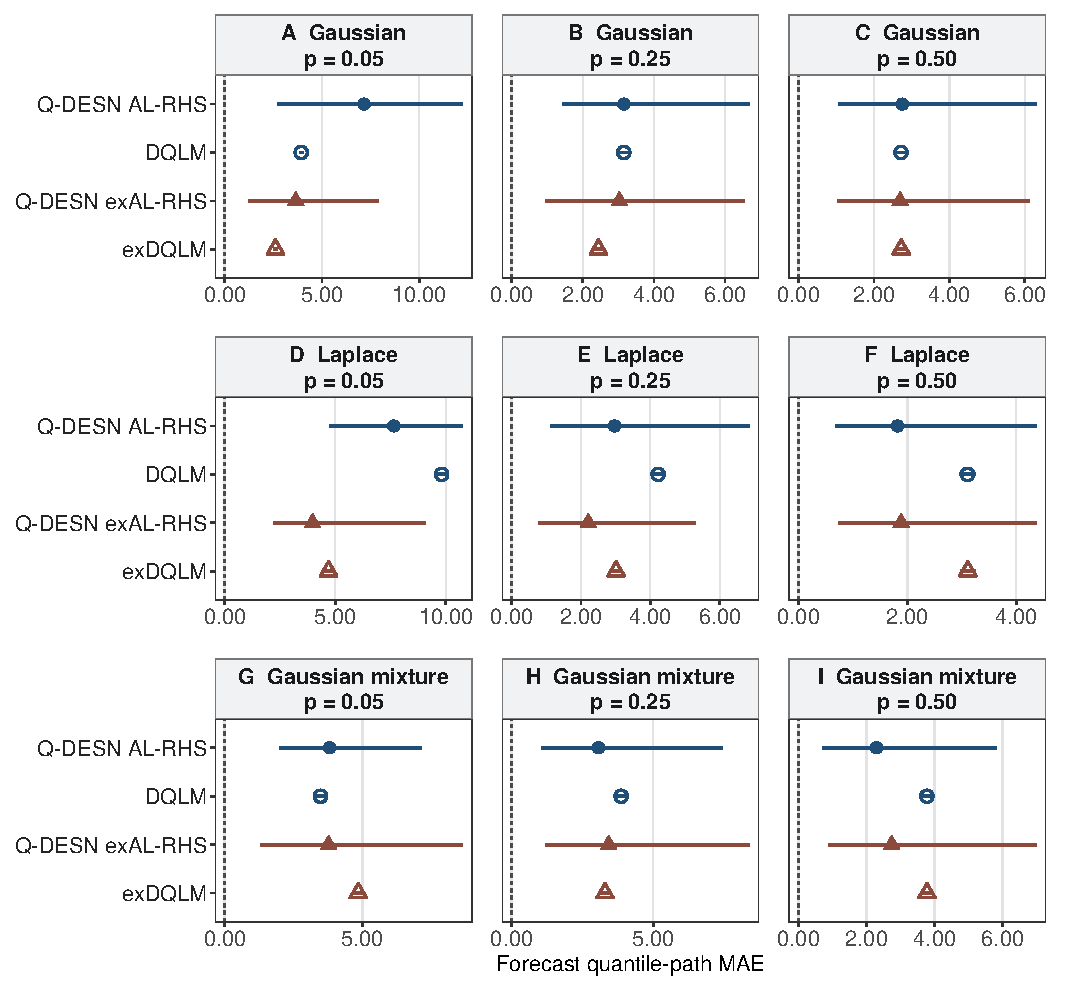
\includegraphics[width=0.98\textwidth]{figures/independent_simulation/qdesn_pro_review_mcmc_forecast_mae.pdf}
\caption{MCMC forecast quantile-path mean absolute error (MAE) in the single-quantile study. Points and equal-tailed 95\% intervals summarize the draw-wise criterion averaged over the forecast pairs. Lower values are better. Navy circles identify \(\AL\) models and muted-brick triangles \(\exAL\) models; filled symbols denote Q--DESN and open symbols their dynamic linear comparators. Panels A--I identify the observation-error family and probability level, with separate horizontal scales. The dashed line marks exact recovery. DESN specifications are criterion-specific; their selection and the forecast-draw construction are documented in the supplement.}
\figalt{Nine panels compare posterior forecast-MAE means and 95 percent
intervals for four models across three observation-error families and three
probability levels. Lower values are better.}
\label{fig:simulation-500obs-mcmc-forecast-mae-intervals}
\end{figure}

\begin{figure}[!htbp]
\centering
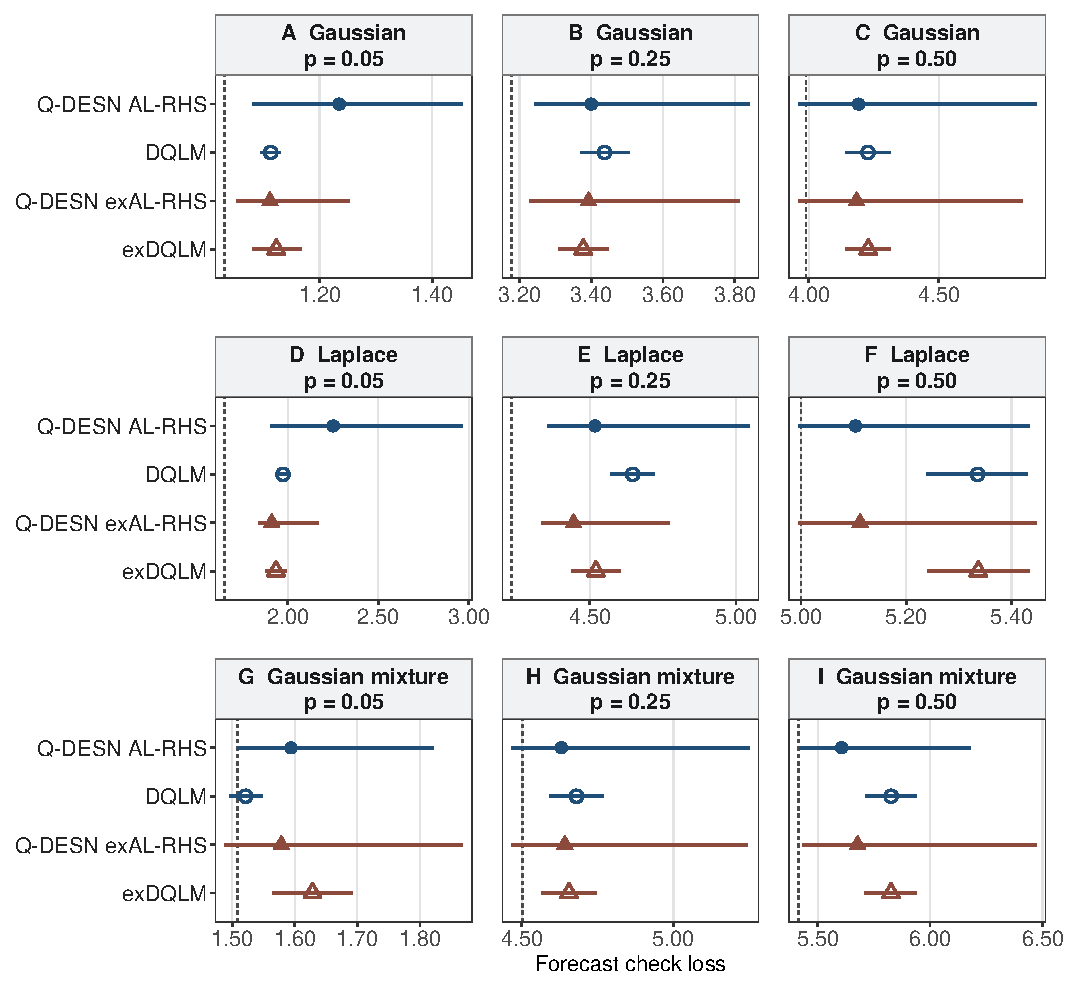
\includegraphics[width=0.98\textwidth]{figures/independent_simulation/qdesn_pro_review_mcmc_forecast_check_loss.pdf}
\caption{MCMC forecast check loss in the single-quantile study. Points and equal-tailed 95\% intervals summarize the draw-wise criterion averaged over the forecast pairs; lower values are better. Model encodings and panels are as in Figure~\ref{fig:simulation-500obs-mcmc-forecast-mae-intervals}. The dashed line marks the population expected check loss at the true conditional quantile. The supplement documents criterion-specific selection and forecast-draw construction.}
\figalt{Nine panels compare posterior forecast-check-loss means and 95 percent
intervals for four models across three observation-error families and three
probability levels. Lower values are better.}
\label{fig:simulation-500obs-mcmc-forecast-check-loss-intervals}
\end{figure}
